\documentclass[12pt]{elsarticle}

\usepackage{lineno,hyperref,notoccite,etoolbox}
\makeatletter
\def\ps@pprintTitle{%
	\let\@oddhead\@empty
	\let\@evenhead\@empty
	\def\@oddfoot{\centerline{\thepage}}%
	\let\@evenfoot\@oddfoot}
\makeatother
\usepackage{setspace}
\singlespacing
\usepackage{mathptmx}
\usepackage{float,wrapfig}
\usepackage[margin=1in]{geometry}
\usepackage{booktabs}
\usepackage{cancel}
\usepackage[fleqn]{amsmath}
\usepackage{amssymb}
\allowdisplaybreaks
\newcommand{\bnumbers}{\begin{enumerate}}
	\newcommand{\enumbers}{\end{enumerate}}
\newcommand{\vs}{\vspace{2mm}}
\newcommand{\beq}{\begin{equation*}}
\newcommand{\eeq}{\end{equation*}}
\newcommand{\rr}[1]{\mbox{#1}}
\newcommand{\longequals}{{=\joinrel=}}
\newcommand{\squared}{$^{2}$}
\newcommand{\subtwo}{$_{2}$}
%tables
\setlength{\arrayrulewidth}{0.5mm}
\setlength{\tabcolsep}{5pt}
\renewcommand{\arraystretch}{1.75}
\newcommand{\fullline}{\noindent\rule{14cm}{0.4pt} \vspace{4mm}}
\usepackage{subfigure}



\begin{document}
\begin{flushright}
	Ember Sikorski\par
	Homework 4\par
	ECE 624\par 
	28 October 2018
\end{flushright}


\begin{enumerate}
\item  Summarize why the amorphous nature of the device material is important to the device function.
\par \vs 
Chen et al. \cite{Chen2018} study the amorphous phase of a GeSbTe alloy used for phase change memory. Similarities are required between the crystalline and amorphous phase to create a fast, reversible switch, while differences between the two phases allow for signal contrast. In the crystalline phase, delocalized electrons give rise to electronic polarizability and, in turn, increase optical reflectivity.
The authors use electron-density-distribution change (EDDC) to show perturbations when an atom is slightly displaced, indicating polarizability of electrons. These results show that 3-atom motifs found in the amorphous phase do exhibit polarizability and thus optoelectronic reflectance.
\vs 
\item Describe the mechanisms that may help or hinder photoconductivity in an amorphous material.
\par \vs 
Photo occurs when holes trapped at D$^{-}$ centers are excited to the valence band\cite{Street1975}:

\begin{equation}
\sigma_{ph} \propto \Delta N \exp \bigg(\frac{-W_{1}}{kT}\bigg) \qquad ,
\end{equation}

where $\Delta N$ is the excess concentration of D$^{0}$ centers. Thus, as the concentration of D$^{0}$ centers increases, photoconductivity decreases. Likewise, at lower values of excess D$^{0}$, photoconductivity increases.
\vs
\item Review Kastner et al. \cite{Kastner} and discuss the following:
	\begin{enumerate}
		\item On the p-level occupation of Figure 1, what does the energy level on the right side correspond to?
		\par \vs
		The energy refers to the amount of energy required to place an electron in the p orbital, with respect to the lone-pair energy.
		\vs 
		\item Explain how the energy listed on the far right is determined for each configuration. 
		\par \vs 
		The energy at first looks like electron affinity:
		\begin{equation}
		EA = E_{vac}-E{CB} \qquad ,
		\end{equation}
		but instead the reference energy is taken as the lone pair energy and the electron is placed in the p orbital. This energy could  be calculated
		\begin{equation}
		E_{b} = -n_{\sigma}E_{b} - n_{\sigma^{*}}(E_{b}-\delta)+(n_{\sigma^{*}}-1)U_{\sigma^{*}}  \qquad ,
		\end{equation}
		where $n$ is the number of electrons placed in the respective bond and $U$ is the respective correlation energy.
		\vs
		\item Provide a drawing of the p-level occupation for the case of a C$_{1}^{+}$. List the energy.
		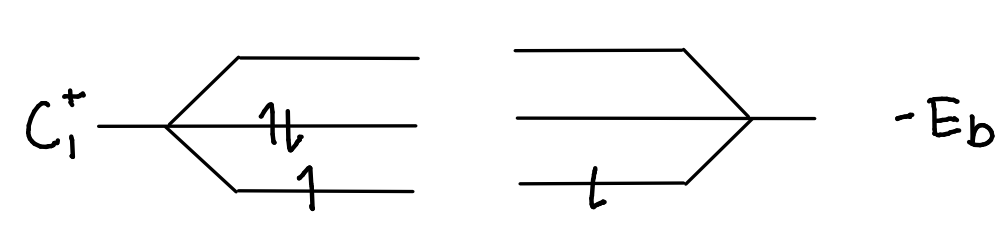
\includegraphics[width=0.5\textwidth]{c}
	\end{enumerate}
\item Describe the type of conduction dominant in an amorphous semiconductor at low temperature, including supporting details.
\par \vs 
Tunneling dominates at low temperatures, as nearest neighbor hopping requires thermal energy for phonon assistance. Instead, variable range hopping takes over where hopping is decided by the greatest probability of success \cite{Yu2001}.
\end{enumerate}


\section*{References}
\bibliography{homework4}
\bibliographystyle{elsarticle-num}


\end{document}  